\chapter{Progettazione}

La fase di progettazione ha avuto l'obiettivo di tradurre i requisiti individuati
nei capitoli precedenti in un'architettura scalabile, accessibile e coerente con
l'identità aziendale. In questa sezione vengono presentate le decisioni
architetturali chiave, il processo metodologico adottato e l'organizzazione
dell'ecosistema di landing pages.

\section{Decisioni architetturali}
Il punto di partenza era una landing page unica, insufficiente per comunicare i
diversi verticali aziendali e raccogliere dati utili a livello di marketing. La
progettazione ha quindi introdotto tre scelte fondamentali:

\begin{itemize}
  \item \textbf{Architettura multi-landing}: adozione di un monorepo (singolo 
  repository contenente tutto il codice delle diverse landing pages) basato su 
  Next.js con sei landing dedicate per i verticali aziendali (/it/home, 
  /it/tech-recruiting/, /it/ai-adoption/, /it/ai-engineering/, 
  /it/tech-media-agency/, /it/jobs/). Include inoltre pagine 
  preesistenti come blog tecnico e pagina contatti, re-integrate 
  nell'architettura unificata. Questa struttura garantisce posizionamento 
  SEO ottimale, riuso di componenti comuni e semplicità di manutenzione.
  
  \item \textbf{Strategia di rendering ibrida}: combina approcci 
  differenziati per tipo di contenuto. Per le sei landing pages principali è 
  stata implementata un'architettura basata su React Server Components 
  (componenti che vengono elaborati interamente sul server prima di essere 
  inviati al browser), seguendo il pattern "Server-First with Selective 
  Hydration". I contenuti statici come hero sections, testi descrittivi e 
  layout vengono renderizzati sul server senza richiedere codice JavaScript 
  nel browser dell'utente. Solo i componenti interattivi specifici (form di 
  contatto, animazioni scroll, tracking analytics) vengono marcati come Client 
  Components e attivati nel browser dopo il caricamento iniziale della pagina, 
  processo chiamato "hydration" (attivazione delle funzionalità interattive). 
  Questo approccio garantisce HTML completo per i motori di ricerca, metriche 
  Core Web Vitals ottimizzate, bundle JavaScript ridotto e Time-to-Interactive 
  (tempo necessario affinché la pagina diventi completamente interattiva) 
  migliorato rispetto a Single Page Application tradizionali.
  
  Il blog tecnico preesistente, re-integrato nel monorepo, implementa Static 
  Site Generation con pre-generazione degli URL degli articoli in fase di build. 
  Le chiamate API al backend Django adottano Incremental Static Regeneration 
  con revalidazione ogni ora, implementando il pattern Stale-While-Revalidate 
  (strategia che serve contenuti memorizzati in cache mentre in background 
  vengono aggiornati con le ultime modifiche), riducendo la dipendenza 
  dall'uptime del backend. La CDN CloudFront 
  distribuisce gli asset statici globalmente, mentre il componente next/image 
  ottimizza automaticamente le immagini con caricamento differito (lazy loading) 
  e conversione in formato WebP. Questa architettura bilancia SEO attraverso 
  HTML completo server-side, performance tramite cache distribuita su CDN, 
  e flessibilità per contenuti multilingua.
  
  \item \textbf{Design system condiviso}: definizione di una libreria di componenti 
  accessibili basata su ShadCN UI (Radix UI primitives) e Tailwind CSS, costruita 
  su linee guida visive aziendali. Garantisce accessibilità WCAG 2.1 AA nativa, 
  customizzazione completa e riutilizzo del codice UI tra le landing.
\end{itemize}

\section{Metodologia di progettazione e collaborazione}
Il progetto di redesign è stato organizzato come una \textbf{macro-release trimestrale},
considerata strategica per l'azienda. La fase di progettazione non si è limitata
alla definizione di scelte tecniche, ma ha previsto un percorso strutturato di
analisi, collaborazione e validazione.

Dopo un'iniziale revisione delle soluzioni esistenti e identificazione dei 
pattern da mantenere o eliminare, il team ha organizzato \textbf{incontri 
interfunzionali} con prodotto, marketing e design per garantire allineamento 
tra esigenze business e soluzioni tecniche. Il rilascio preliminare delle 
landing a un gruppo ristretto di stakeholder interni ha permesso di raccogliere 
feedback e iterare rapidamente sulle ottimizzazioni necessarie.

L'intero processo è stato gestito con \textbf{approccio Agile} strutturato:

\begin{itemize}
  \item Sprint bisettimanali con planning e retrospettive dedicate.
  \item Daily standup per allineamento quotidiano del team.
  \item Progettazione responsive fin dall'inizio per garantire user experience 
        coerente su desktop, tablet e mobile.
\end{itemize}

Questa metodologia ha consentito di ridurre i rischi, migliorare la qualità
finale e assicurare che le landing rispondessero realmente ai bisogni degli utenti
e dell'azienda.

\section{Processo di design e design system}
Il design system è stato sviluppato in stretta collaborazione con il team UX/UI,
a partire da wireframe validati con il product team fino a mockup
high-fidelity realizzati in Figma. Il processo ha incluso la definizione di 
\textbf{design tokens comuni} (colori, tipografia, spaziatura) condivisi tra 
Figma e configurazioni Tailwind CSS di progetto, seguita dalla creazione di 
\textbf{componenti modulari} con varianti responsive per garantire consistenza 
visiva e riutilizzo tra le sei landing pages principali.

L'architettura componenti ha permesso di standardizzare elementi ricorrenti 
garantendo il riutilizzo di molto del codice UI tra le diverse landing. Questo 
approccio ha permesso di ridurre i tempi di sviluppo, garantire coerenza tra 
design e implementazione e abilitare una rapida iterazione.

Come mostrato in Figura~\ref{fig:design-system}, il design system include 
componenti modulari standardizzati (tipografia, colori, spacing, componenti UI) 
che assicurano coerenza visiva e riutilizzo del codice tra tutte le landing pages.

\begin{figure}[h!]
    \centering
    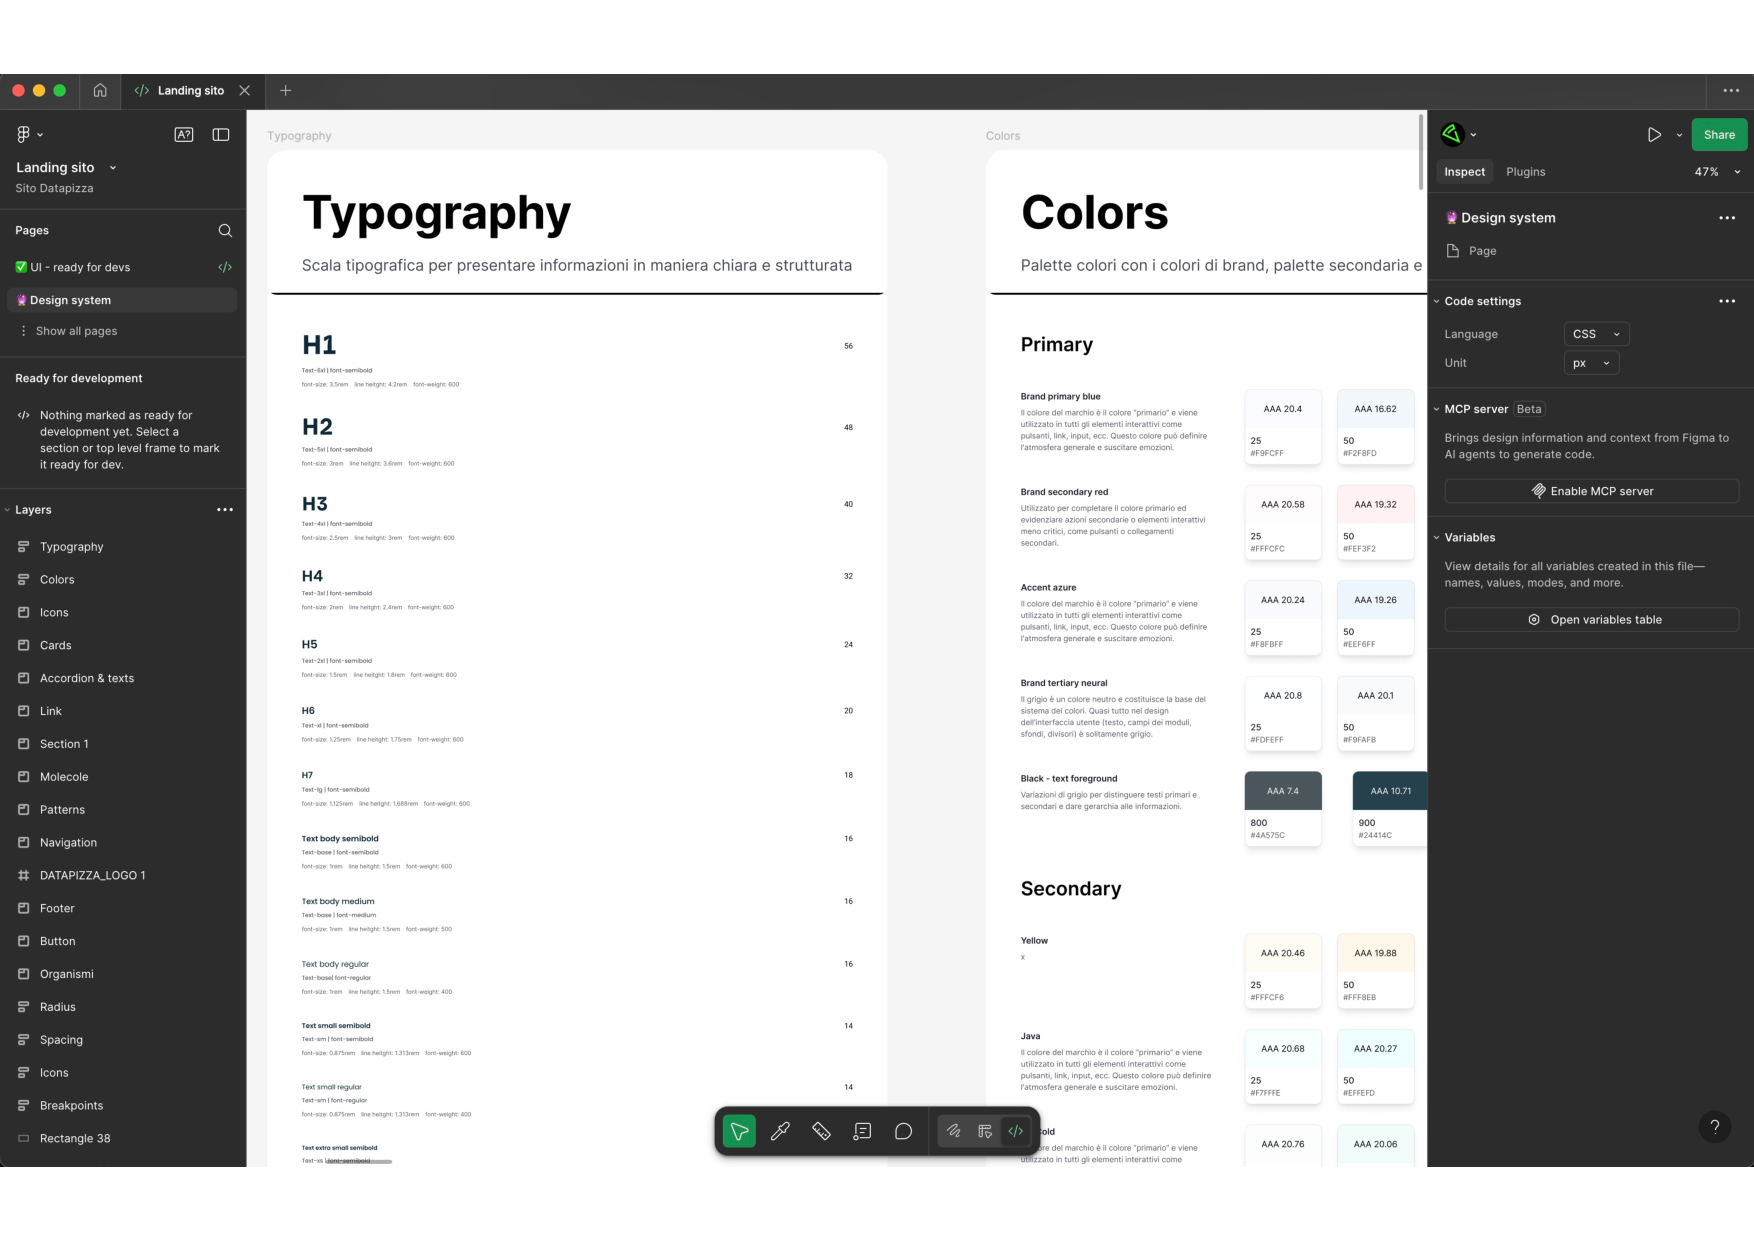
\includegraphics[width=\textwidth]{chapters/figures/design-system.pdf}
    \caption{Esempi di componenti principali del design system.}
    \label{fig:design-system}
\end{figure}

\clearpage
\section{Architettura delle landing pages}
L'ecosistema è stato progettato con una struttura comune di base (\textit{navbar}, 
\textit{footer}) e con personalizzazioni specifiche per ciascun verticale. 
Ogni landing è stata progettata con registro linguistico e UX mirati per target 
specifici:

\begin{itemize}
  \item \textbf{Home Page} (/it/): hub centrale con panoramica generale dei 
  4 verticali e routing intelligente verso servizi specifici per visitatori generici.
  
  \item \textbf{Tech Recruiting} (/it/tech-recruiting/): landing B2B con registro 
  consulenziale, layout pulito, form contatto con campi aziendali e CTA demo-oriented 
  (``Richiedi demo``, ``Contatta team``) per aziende in cerca di talenti tech.
  
  \item \textbf{Tech Community} (/it/tech-media-agency/): linguaggio informale, 
  elementi visuali orientati alla cultura developer, CTA engagement per newsletter 
  ``Commit`` e social proof con 500k+ iscritti per developer e tech enthusiast.
  
  \item \textbf{AI Adoption} (/it/ai-adoption/): registro professionale B2B 
  enterprise, focus upskilling organizzativo con case studies aziendali e CTA 
  consulenza personalizzata per HR e management.
  
  \item \textbf{AI Engineering} (/it/ai-engineering/): showcase framework 
  proprietario ``Datapizza AI`` con gallery progetti (Copiloti Sales/HR/Legal/Customer) 
  e CTA demo tecnica per CTO e IT Decision Makers.
  
  \item \textbf{Jobs Platform} (/jobs/): stile diretto B2C, call-to-action 
  immediate (``Cerca lavoro``, ``Candidati ora``), esperienza mobile-first con 
  trasparenza salary (RAL sempre visibile), Tech Buddy matching e zero ghosting 
  policy per candidati in cerca di opportunità tech.
\end{itemize}

Questa differenziazione per target ha permesso di ottimizzare i tassi di 
conversione specifici per ciascun servizio, garantendo messaggi mirati e 
customer journey personalizzati.

\clearpage
La Figura~\ref{fig:jobs-desktop} mostra il layout desktop della Jobs Platform, 
progettato per massima trasparenza salariale (RAL sempre visibile in evidenza) 
e navigazione intuitiva con filtri di ricerca prominenti.
\begin{figure}[h!]
    \centering
    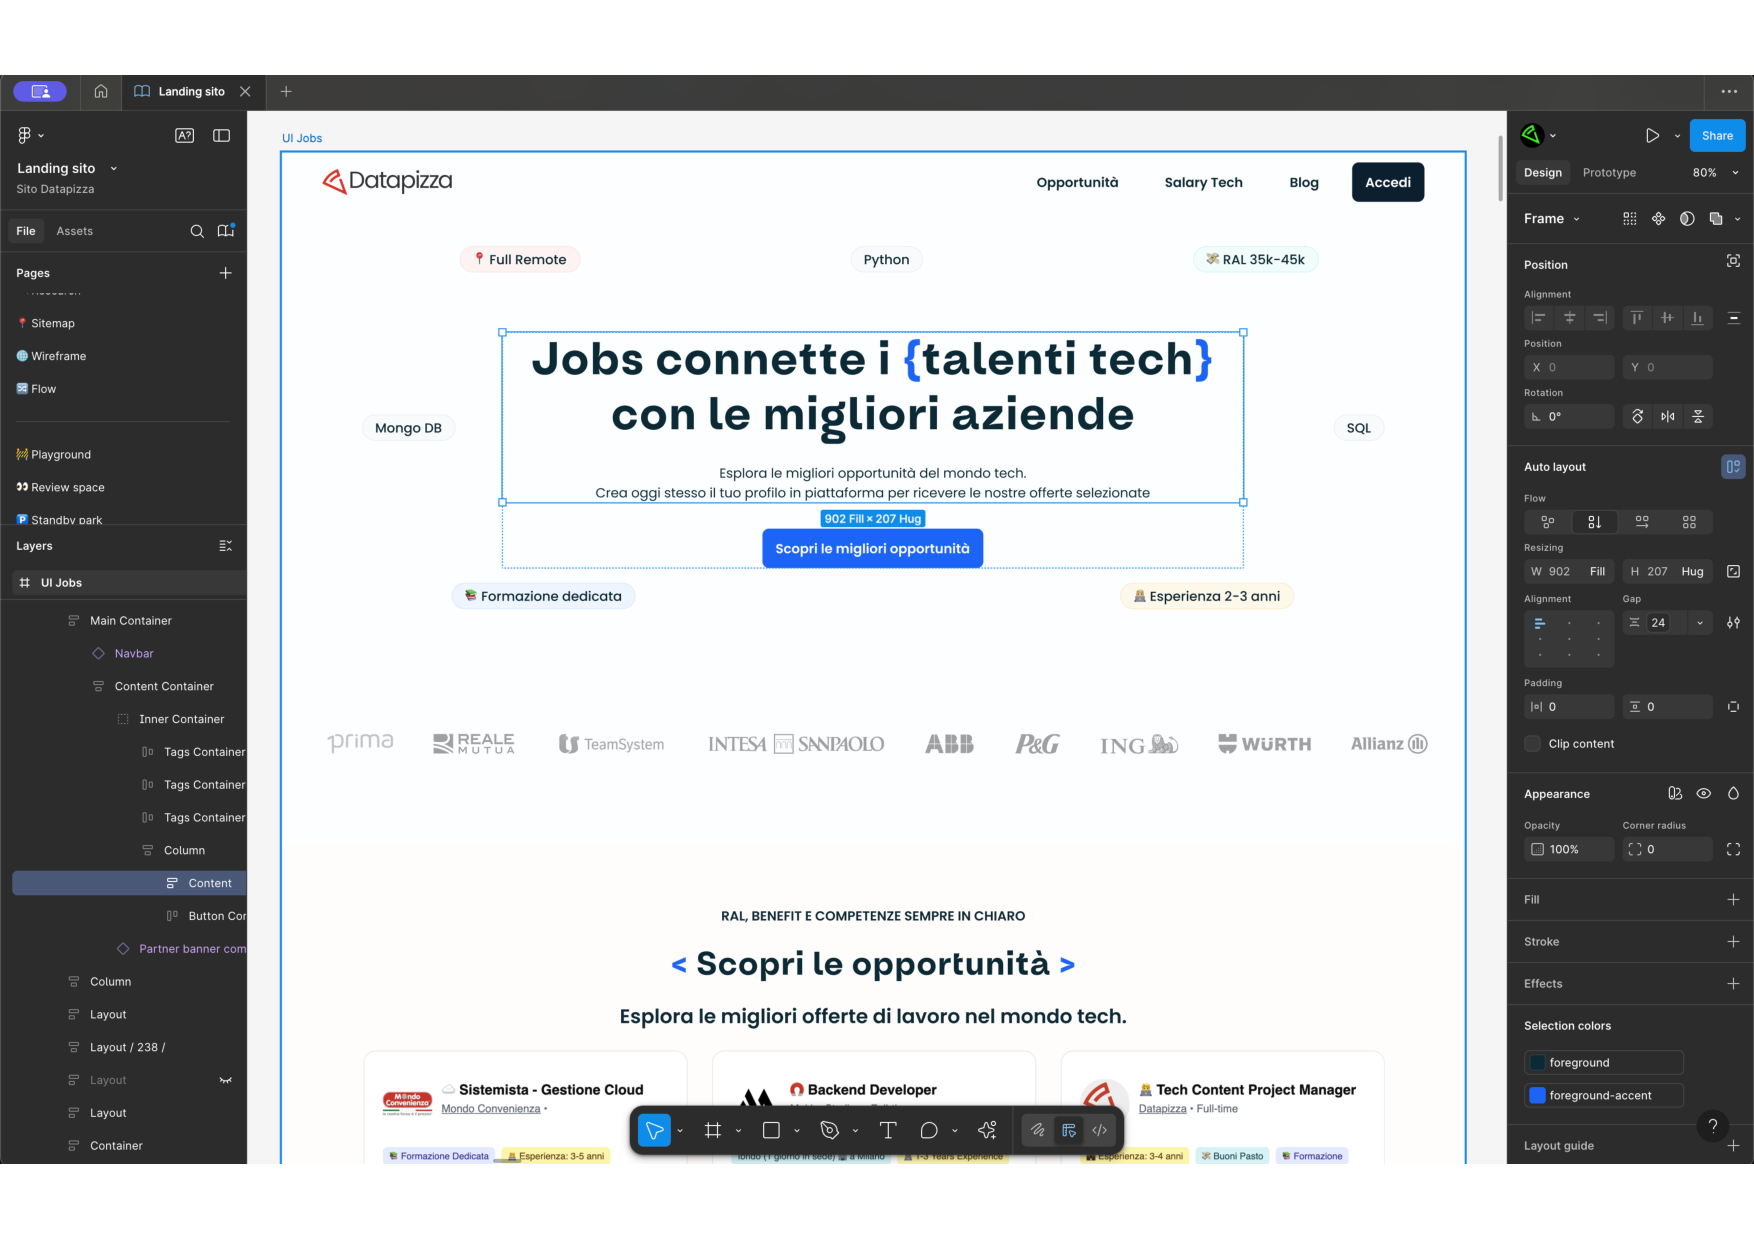
\includegraphics[width=1.06\textwidth]{chapters/figures/mockup.pdf}
    \caption{Mockup desktop della Jobs Platform.}
    \label{fig:jobs-desktop}
\end{figure}

\clearpage
La versione mobile della landing AI Engineering (Figura~\ref{fig:ai-eng-mobile}) 
privilegia un design minimale con call-to-action ben visibili, mantenendo 
coerenza cromatica e strutturale con la versione desktop.
\begin{figure}[h!]
    \centering
    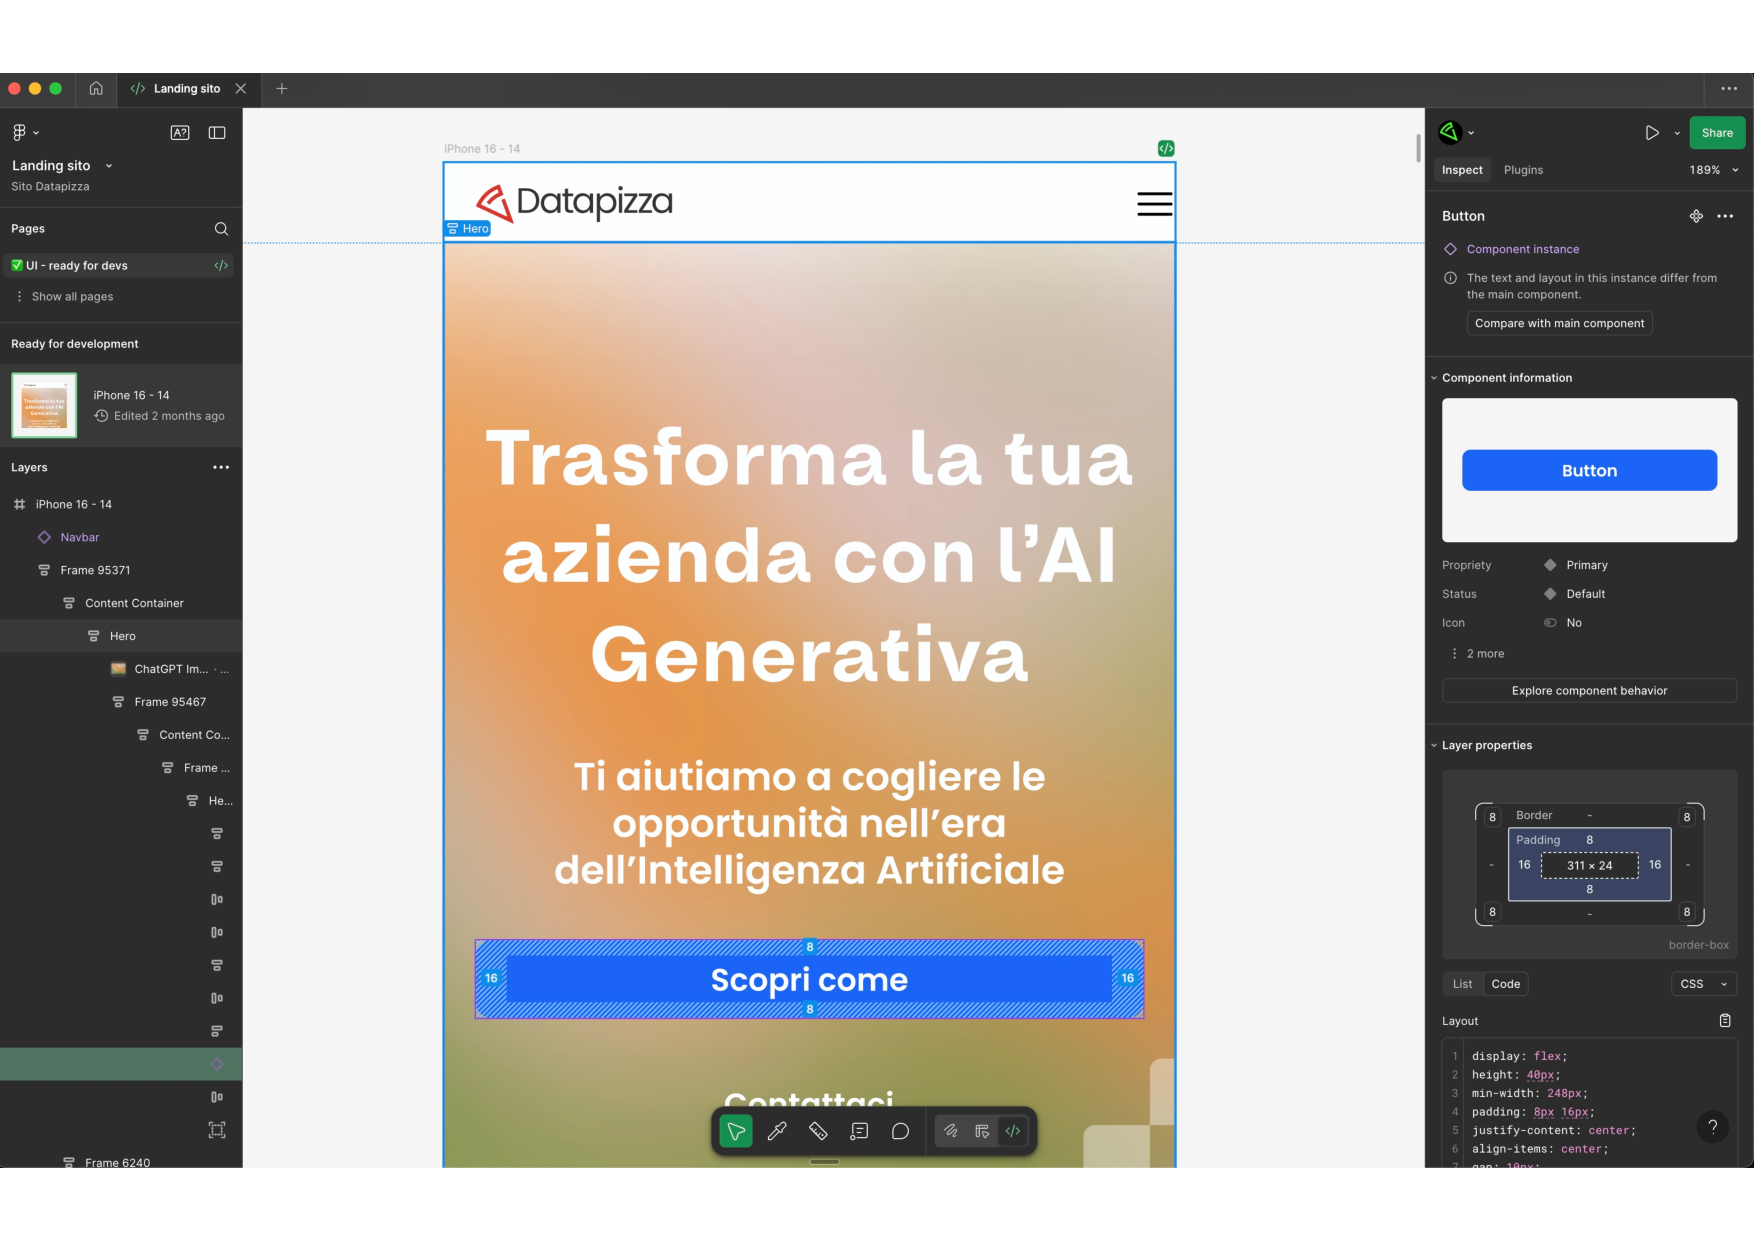
\includegraphics[width=1.06\textwidth]{chapters/figures/mockup2.pdf}
    \caption{Mockup mobile della landing AI Engineering.}
    \label{fig:ai-eng-mobile}
\end{figure}
\clearpage

\section{Tracking e misurabilità}
Il sistema di tracking è stato progettato per migliorare l'implementazione 
precedentemente presente, supportando funnel di conversione specifici per ogni 
verticale. L'integrazione con Mixpanel consente di tracciare page view, 
interazioni e conversioni con granularità maggiore rispetto alla soluzione unica 
precedente.

\subsection{Event taxonomy e funnel}
L'architettura tracking implementa una \textbf{tassonomia strutturata} 
su tre livelli gerarchici. Il primo livello monitora gli eventi di 
visualizzazione pagina (quando un utente carica una landing), il secondo 
traccia le interazioni (click su pulsanti, scroll progressivo della pagina, 
visualizzazione sezioni specifiche), mentre il terzo cattura le conversioni 
finali (compilazione form contatto, iscrizione newsletter).

Questa classificazione permette di analizzare \textbf{funnel di conversione 
differenziati per verticale}. Per le landing B2B (Recruiting, AI Adoption, 
AI Engineering), il percorso completo va dalla visualizzazione iniziale 
fino al click su call-to-action, apertura del form di contatto e invio 
dei dati per generare lead commerciali qualificati. La piattaforma Jobs 
B2C monitora invece il flusso dalla visualizzazione della landing all'utilizzo 
della ricerca offerte, click su posizione lavorativa e reindirizzamento 
verso il prodotto Datapizza Jobs per completare la candidatura. La landing 
Community traccia il percorso dall'arrivo sulla pagina fino al click sul 
pulsante di iscrizione e conferma dell'iscrizione alla newsletter ``Commit``.

Questa segmentazione consente analisi specifiche per ottimizzazione delle 
conversioni e identificazione dei punti di abbandono (drop-off) nel customer 
journey, permettendo di migliorare continuamente l'esperienza utente per 
ciascun target.

\subsection{GDPR compliance}
Particolare attenzione è stata data alla conformità normativa europea con 
approccio privacy-by-design: consenso esplicito tramite cookie banner prima 
di inizializzazione Mixpanel, anonimizzazione automatica degli indirizzi IP 
e gestione opt-out utente.

\bigskip
In sintesi, la progettazione ha fornito una base metodologica e architetturale 
solida che ha guidato in modo diretto le fasi di sviluppo, deployment e verifica 
descritte nei capitoli successivi.